%=======================================================================
%  41277 Control Design -- Task 5 final project demonstration
%  5-minute presentation: three parts, about 100 s per speaker.
%  Build: latexmk -pdf demo_slides.tex   (pdflatex; figures in figures/)
%  Slides after \appendix are backup for the questions, not presented.
%=======================================================================
\documentclass[aspectratio=169,10pt]{beamer}
\usetheme[progressbar=frametitle,numbering=fraction,block=fill]{metropolis}
\usepackage{amsmath,amssymb,bm}
\usepackage{booktabs}
\usepackage{tikz}
\usetikzlibrary{positioning,arrows.meta}

\definecolor{uts}{HTML}{1F4E9A}
\definecolor{ok}{HTML}{1F7A4D}
\definecolor{fix}{HTML}{B35A00}
\setbeamercolor{frametitle}{bg=uts}
\setbeamercolor{progress bar}{fg=fix}
\setbeamercolor{block title}{bg=uts!12,fg=uts}
\setbeamercolor{block body}{bg=uts!5}
\setbeamerfont{itemize/enumerate body}{size=\small}
\setbeamerfont{itemize/enumerate subbody}{size=\small}
\setbeamerfont{frametitle}{size=\large}

% Speaker tag in the bottom-left corner of a slide
\newcommand{\speaker}[1]{%
  \begin{tikzpicture}[remember picture,overlay]
    \node[anchor=south west,font=\scriptsize\bfseries,text=white,fill=fix,
          rounded corners=2pt,inner sep=3pt] at ([xshift=6pt,yshift=5pt]current page.south west) {#1};
  \end{tikzpicture}}

\title{Balancing the QUBE-Servo~2 rotary inverted pendulum}
\subtitle{Two digital control systems, from model to hardware}
\author{Jaylen Avtarovski \and Rhyse Williams \and Elina Kim}
\institute{41277 Control Design · Task 5 final project demonstration · UTS, Spring 2026}
\date{}

\begin{document}

\maketitle

%=======================================================================
\begin{frame}{The plant, and three facts that shape both designs}
\speaker{Part 1 · Modelling}
\begin{columns}[T,onlytextwidth]
\column{0.46\textwidth}
\textbf{Model from first principles}
\begin{itemize}
  \item Euler--Lagrange in $\theta$ (arm) and $\alpha$ (pendulum, 0 upright)
  \item Motor torque $\tfrac{k_t}{R_m}(V_m - k_m\dot\theta)$, inductance neglected
  \item Linearised at upright, $x=[\theta\ \alpha\ \dot\theta\ \dot\alpha]^T$
\end{itemize}
\textbf{Sensors and sampling}
\begin{itemize}
  \item Encoders $0.176^\circ$/count; $\alpha$ counted backwards, corrected in the controller
  \item $T_s=1$\,ms: $\omega_cT_s\approx0.02$
\end{itemize}
\column{0.51\textwidth}
\begin{block}{From the transfer functions}
\footnotesize
\vspace{-4pt}
\begin{align*}
G_\theta&=\frac{18.07(s-8.97)(s+12.7)}{s(s-9.95)(s+4.02)(s+17.6)}\\
G_\alpha&=\frac{17.86\,s}{(s-9.95)(s+4.02)(s+17.6)}
\end{align*}
\begin{enumerate}
  \item \textbf{Unstable:} pole at $+9.95$ (falls in $\approx0.1$\,s)
  \item \textbf{Non-minimum phase:} zero at $+8.97$; the arm moves the wrong way first
  \item \textbf{Zero at $s=0$ in $G_\alpha$:} a pendulum loop alone can't hold the arm
\end{enumerate}
\end{block}
\small One voltage, two outputs: both designs need a pendulum loop \emph{and} an arm loop.
\end{columns}
\end{frame}

%=======================================================================
\begin{frame}{CS1 (frequency domain): two filtered-PD loops, by pole placement}
\speaker{Part 2 · CS1}
\begin{columns}[T,onlytextwidth]
\column{0.47\textwidth}
\centering
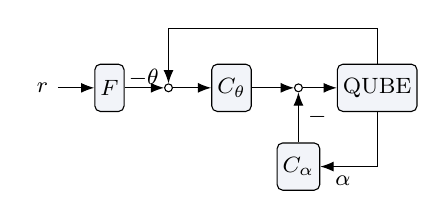
\begin{tikzpicture}[>=Latex,font=\footnotesize,
    b/.style={draw,rounded corners=2pt,minimum height=6mm,inner sep=2pt,fill=uts!6}]
  \node (r) at (0,0) {$r$};
  \node[b] (F) at (0.85,0) {$F$};
  \node[draw,circle,inner sep=1pt] (s1) at (1.6,0) {};
  \node[b] (Ct) at (2.4,0) {$C_\theta$};
  \node[draw,circle,inner sep=1pt] (s2) at (3.25,0) {};
  \node[b] (P) at (4.25,0) {QUBE};
  \node[b] (Ca) at (3.25,-1.0) {$C_\alpha$};
  \draw[->] (r) -- (F); \draw[->] (F) -- (s1); \draw[->] (s1) -- (Ct);
  \draw[->] (Ct) -- (s2); \draw[->] (s2) -- (P);
  \draw[->] (P.north) -- ++(0,0.45) -| node[pos=0.95,left]{$-\theta$} (s1.north);
  \draw[->] (P.south) |- node[pos=0.8,below]{$\alpha$} (Ca.east);
  \draw[->] (Ca.north) -- node[right]{$-$} (s2.south);
\end{tikzpicture}
\[
C_i(s)=K_{p,i}+K_{d,i}\tfrac{Ns}{s+N},\quad N=60
\]
\begin{itemize}
  \item Derivative: lead to stabilise $+9.95$
  \item $N$: limits gain on quantisation noise
  \item Everything in \emph{one} MATLAB Function block at 1\,ms
\end{itemize}
\column{0.5\textwidth}
\textbf{Design steps}
\begin{enumerate}
  \item Specs to poles: $\zeta=0.7$ ($M_p=4.6\%$), $\omega_n=8$ ($t_s\approx0.71$\,s), $-19.2$, $-25.6$
  \item Degree-5 polynomial with a fixed $s^4$ term: fifth pole forced to $-15.7$
  \item Match $s^3\ldots s^0$: 4 linear equations, 4 gains\\
        $K_{p\theta}=-3.99$, $K_{d\theta}=-1.72$, $K_{p\alpha}=42.9$, $K_{d\alpha}=2.38$
  \item Negative arm gains: the RHP zero
  \item $F(s)=\frac{2.23}{s+2.23}\cdot\frac{3}{s+3}$ cancels the slow zero at $-2.23$: less overshoot, same poles
\end{enumerate}
\end{columns}
\end{frame}

%=======================================================================
\begin{frame}{CS1: verified in frequency, discretised with Tustin}
\speaker{Part 2 · CS1}
\begin{columns}[T,onlytextwidth]
\column{0.53\textwidth}
\centering
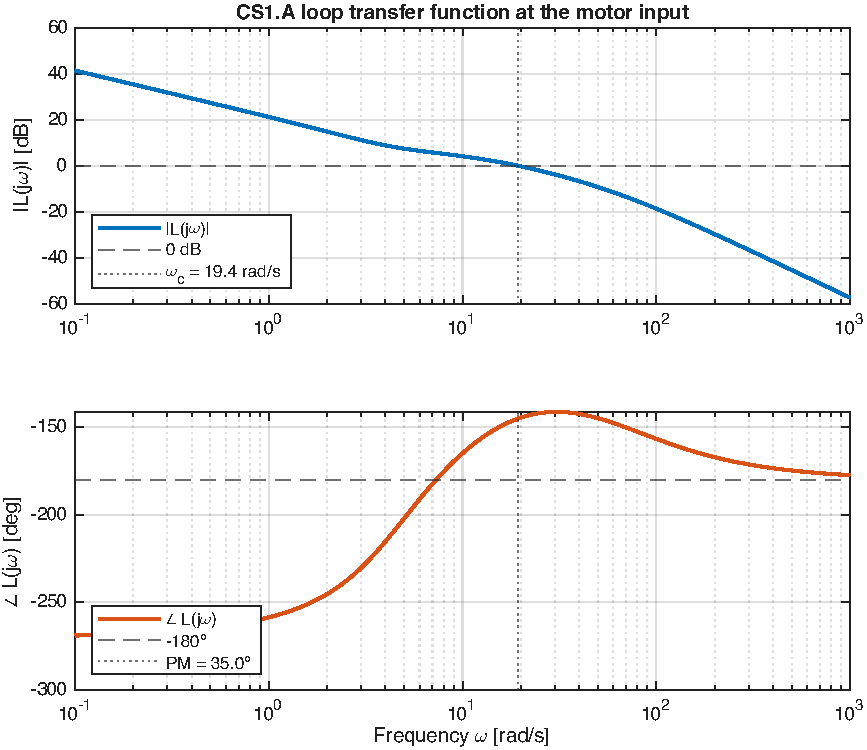
\includegraphics[height=0.72\textheight,width=\linewidth,keepaspectratio]{figures/cs1a_bode}
\column{0.44\textwidth}
\textbf{Loop broken at the motor input}
\begin{itemize}
  \item $\omega_c=19.4$\,rad/s, phase margin $34^\circ$
  \item Gain margin is a band, $0.53\times$ to $68\times$: one unstable pole, so Nyquist needs one encirclement
  \item Delay margin 31\,ms, $M_s=1.66$
\end{itemize}
\textbf{Discretisation}
\begin{itemize}
  \item Tustin: stable $C(s)\Rightarrow$ stable $C(z)$
  \item Filter pole $0.94175$ vs $e^{-NT_s}=0.94176$
  \item Arm loop since upgraded to a PID (integrator, zero at $-0.5$) for the friction offset
\end{itemize}
\end{columns}
\end{frame}

%=======================================================================
\begin{frame}{CS1 results: meets the specs, rejects bumps on the QUBE}
\speaker{Part 2 · CS1}
\begin{columns}[T,onlytextwidth]
\column{0.49\textwidth}
\centering
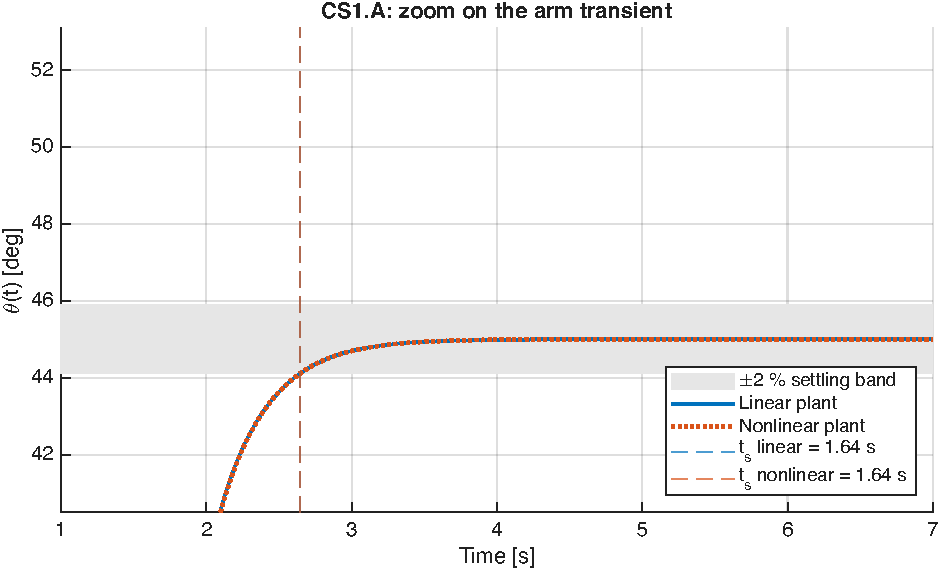
\includegraphics[height=0.55\textheight,width=\linewidth,keepaspectratio]{figures/cs1a_sim_zoom}\\
\small Simulation, $45^\circ$ step: \textbf{0\% overshoot}, \textbf{$t_s=1.64$\,s}
\column{0.49\textwidth}
\centering
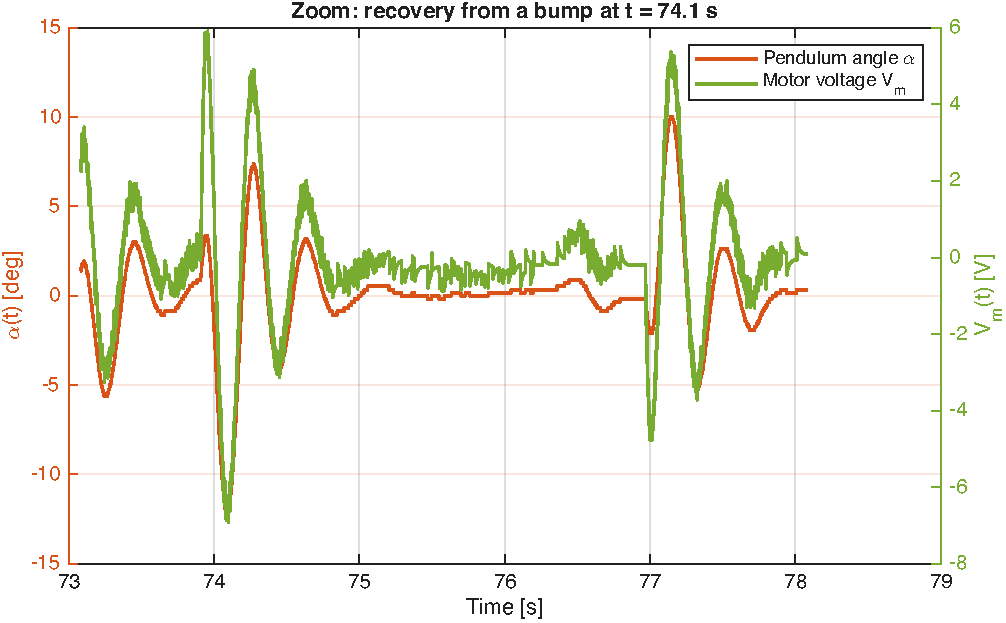
\includegraphics[height=0.55\textheight,width=\linewidth,keepaspectratio]{figures/hw_cs1a_bump}\\
\small QUBE: balanced 171\,s; $12^\circ$ bump recovered in about 3.5\,s
\end{columns}
\vspace{4pt}
\small Undershoot first (the RHP zero); linear and nonlinear overlap; $\pm1$\,V chatter from quantised encoders.
\end{frame}

%=======================================================================
\begin{frame}{CS2 (time domain): state feedback with an observer}
\speaker{Part 3 · CS2}
\begin{columns}[T,onlytextwidth]
\column{0.55\textwidth}
\textbf{Every 1\,ms, in one MATLAB Function block}
\small
\begin{align*}
r_f &\leftarrow r_f+\tfrac{T_s}{\tau}(r-r_f),\quad x^*=[r_f\ 0\ 0\ 0]^T\\
u &= \operatorname{sat}_{\pm10}\big[-F(\hat x-x^*)-F_i\,x_i\big]\\
x_i &\leftarrow x_i+T_s(\theta-r)\ \ \text{within }\pm2^\circ\\
\hat x &\leftarrow A\hat x+Bu+L_o(y-C\hat x)
\end{align*}
\begin{itemize}
  \item Controllable and observable: both ranks $=4$
  \item Observer estimates $\dot\theta$, $\dot\alpha$ from the model, without differentiating encoders
  \item Poles in $s$, mapped by $z=e^{sT_s}$; $F$, $F_i$ by \texttt{place} on $[x;\,x_i]$
\end{itemize}
\column{0.42\textwidth}
\centering
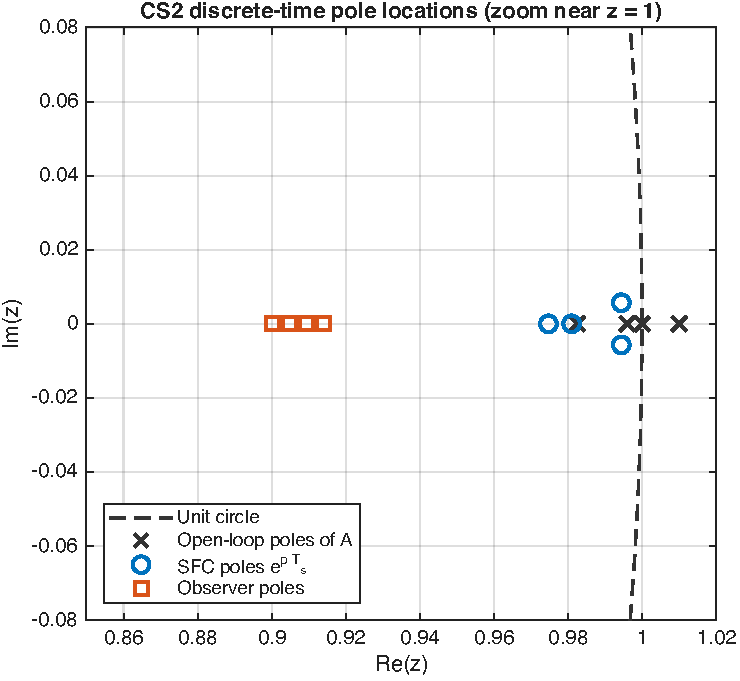
\includegraphics[height=0.5\textheight,width=\linewidth,keepaspectratio]{figures/cs2_zplane}\\
\footnotesize
\begin{tabular}{@{}ll@{}}
\toprule
SFC & $\zeta=0.7$, $\omega_n=8$; $-19.2$, $-25.6$\\
Integrator & $-1$\\
Observer & $-90$ to $-105$ ($4\times$ fastest)\\
\bottomrule
\end{tabular}
\end{columns}
\end{frame}

%=======================================================================
\begin{frame}{CS2: what the hardware taught us}
\speaker{Part 3 · CS2}
\begin{columns}[T,onlytextwidth]
\column{0.52\textwidth}
\footnotesize
\begin{tabular}{@{}p{0.24\linewidth}p{0.71\linewidth}@{}}
\toprule
\textbf{Problem} & \textbf{Cause and fix}\\
\midrule
Wouldn't balance & Encoder signs were wrong, and the DP2 poles ($\omega_n=2.5$) need motor gain $\ge0.87\times$; hardware data suggests it's lower. Signs fixed and CS1's bandwidth: stable for \textcolor{ok}{\textbf{0.45--5.3$\times$}}\\[3pt]
Arm offset & Friction dead band: conditional integral with anti-windup\\[3pt]
Fell when bumped & Integrator pole $-8$ tripled the gains, so bumps hit $\pm10$\,V. Pole $-1$: \textcolor{ok}{\textbf{197 vs 119\,$^\circ$/s}} kicks recovered\\
\bottomrule
\end{tabular}
\column{0.45\textwidth}
\centering
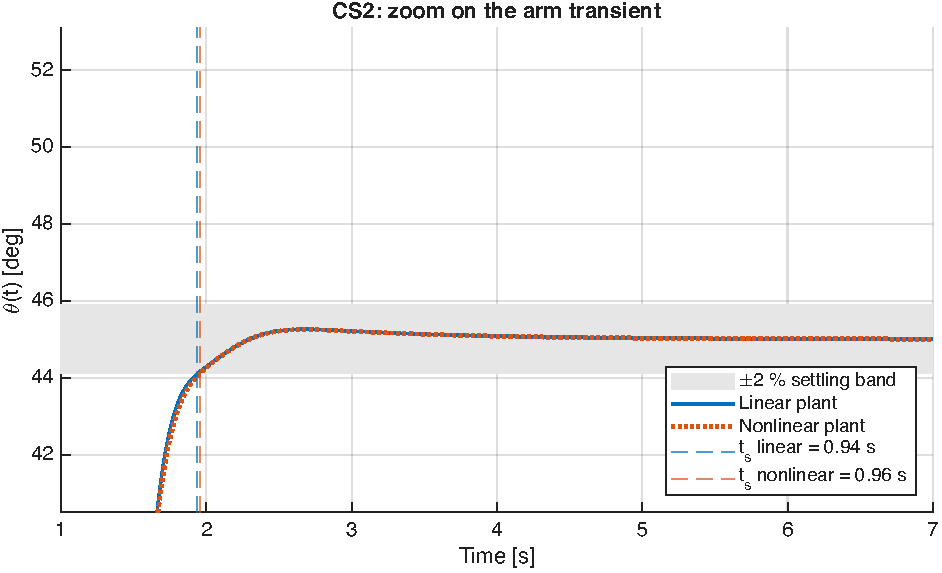
\includegraphics[height=0.52\textheight,width=\linewidth,keepaspectratio]{figures/cs2_sim_zoom}\\
\small Simulation, $45^\circ$ step: \textbf{0.6\% overshoot}, \textbf{$t_s=0.96$\,s}
\end{columns}
\vspace{4pt}
\small Damping: $\zeta=0.7$ dominant pair; reference filter and conditional integral stop windup overshoot (44\% otherwise).
\end{frame}

%=======================================================================
\begin{frame}{Comparison, then the live demo}
\speaker{Part 3 · CS2}
\begin{columns}[T,onlytextwidth]
\column{0.55\textwidth}
\centering
\small
\begin{tabular}{@{}lcc@{}}
\toprule
$45^\circ$ step, nonlinear sim. & \textbf{CS1} & \textbf{CS2}\\
\midrule
Overshoot (spec $<15\%$) & 0\% & 0.6\%\\
Settling (spec $<5$\,s) & 1.64\,s & 0.96\,s\\
Peak $|V_m|$ & 0.8\,V & 1.6\,V\\
Peak $|\alpha|$ & $2.4^\circ$ & $4.6^\circ$\\
Stable motor gain & $0.53$--$68\times$ & $0.45$--$5.3\times$\\
Friction offset & arm PID & integral\\
\bottomrule
\end{tabular}
\column{0.42\textwidth}
\textbf{Lessons}
\begin{itemize}
  \item Passing in simulation isn't enough: margin to the weaker real motor decided both designs
  \item High gains saturate on bumps
  \item Check sensor conventions: $\alpha$ was reversed
\end{itemize}
\begin{block}{Live demo}
\small Simulation, then both controllers on the QUBE: balance, step, bump.
\end{block}
\end{columns}
\end{frame}

%=======================================================================
\appendix
\begin{frame}[standout]
Backup slides for questions
\end{frame}

\begin{frame}{Backup: sampling time and the $s\to z$ mapping}
\begin{columns}[T,onlytextwidth]
\column{0.48\textwidth}
\textbf{Why $T_s=1$\,ms}
\begin{itemize}
  \item The template's rate on the Teensy (1\,kHz)
  \item Fastest open-loop pole $-17.6$: $|\lambda|T_s\approx0.018\ll1$
  \item $2\pi/T_s\approx6280$\,rad/s, over $300\times$ CS1's $\omega_c$
  \item Observer $-105$: about 10 samples per time constant
  \item Faster only makes derivatives noisier ($0.176^\circ$ steps)
\end{itemize}
\column{0.48\textwidth}
\textbf{$z=e^{sT_s}$}, exact for ZOH since $A=e^{A_cT_s}$
\begin{itemize}
  \item $-5.6\pm5.71j\to0.9944\pm0.0057j$
  \item $-19.2\to0.9810$, $-25.6\to0.9747$, $-1\to0.9990$
  \item Observer: $0.914$ to $0.900$
  \item Unstable $+9.95\to1.0100$, outside the circle
  \item Left half-plane to inside the circle; larger $|s|$ gives smaller $|z|$
\end{itemize}
\end{columns}
\end{frame}

\begin{frame}{Backup: observer poles, and overshoot without moving poles}
\begin{columns}[T,onlytextwidth]
\column{0.48\textwidth}
\textbf{Observer poles $-90$ to $-105$}
\begin{itemize}
  \item About $4\times$ the fastest SFC pole: converges first
  \item Distinct and real: \texttt{place} allows multiplicity $\le\operatorname{rank}C=2$
  \item Not faster: a larger $L_o$ passes quantisation into the velocity estimates
  \item $L_o$ = \texttt{place(A',C',exp(po\_s*ts))'} by duality
\end{itemize}
\column{0.48\textwidth}
\textbf{Less overshoot, same poles}
\begin{itemize}
  \item Shape the reference path outside the loop: the characteristic equation is unchanged
  \item CS1: $F(s)$ cancels the closed-loop zero at $-2.23$
  \item CS2: reference filter $\tau=0.2$\,s, reference enters through $x^*$, integral only within $\pm2^\circ$
\end{itemize}
\end{columns}
\end{frame}

\begin{frame}[fragile]{Backup: new targets during the demo}
\begin{columns}[T,onlytextwidth]
\column{0.5\textwidth}
\textbf{CS2}, in \texttt{params\_CS2.m}:
\begin{verbatim}
OS_target = 10;   % [%]
ts_target = 2;    % [s]
\end{verbatim}
\small $\zeta=\frac{-\ln M_p}{\sqrt{\pi^2+\ln^2M_p}}$, $\omega_n=\frac{4}{\zeta t_s}$; the fast and observer poles scale with $\omega_n$. Then \texttt{run\_CS2} and rebuild \texttt{hw\_CS2}.
\column{0.46\textwidth}
\small \textbf{CS1}: change \texttt{candidate\_wn} and \texttt{candidate\_zeta} in \texttt{params\_CS1A\_candidate.m}; polynomial matching recomputes all four gains.
\begin{block}{Watch out}
\footnotesize A slower $t_s$ target is fragile (10\%, 2\,s needs motor gain $\ge0.81\times$), and "$t_s<X$" is met by any faster design too. For under about 1\,s, shorten \texttt{ref\_tau}.
\end{block}
\end{columns}
\end{frame}

\begin{frame}{Backup: CS1 root locus}
\centering
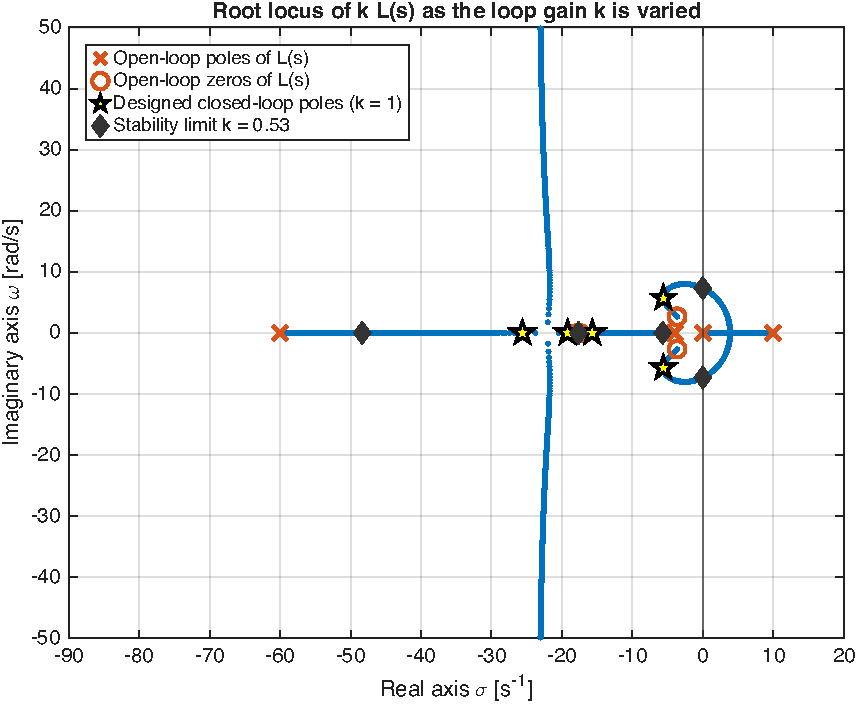
\includegraphics[height=0.72\textheight,width=\linewidth,keepaspectratio]{figures/cs1a_rlocus}\\
\small Branches from $+9.95$ and $0$ cross into the left half-plane at $k=0.53$, the lower gain margin; stars mark the designed poles.
\end{frame}

\end{document}
